\subsection{Spectral Clustering}
\textit{written by M.A.}\\

Spectral clustering is an unsupervised learning algorithm. It is a popular clustering algorithm and is simple to implement \cite{von2007tutorial} Each data point is treated as a graph-node and performs the clustering problem into a graph-partitioning problem \cite{spectral-website}. The affinity rather then the absolute location (i.e. k-means) determines what points are set in which cluster. It is important to mention that there is not made any assumption about the shape or form of the clusters \cite{spectral-website}. \newline

The algorithm consists of the following basic steps \cite{von2007tutorial,spectral-website}: \newline
1.	The construction of a similarity graph : \newline
During this step an undirected graph G = (V,E) with a vertex set V = {v1, v2,… vn} = 1,2,…n observations is being created. This graph is built in the form of an adjaceny matrix which has the similarity between each vertex as its elements. 
There are different options to compute that: The adjacency matrix can be built as an Epsilon-neighbourhood graph, K-Nearest Neighbours strategy or a fully-connected graph. \newline

1.1	The Epsilon-neighbourhood graph sets the parameter epsilon. Then each point is connected to all the points, which lie in the epsilon -radius. The graph which is built in this case is an undirected and unweighted graph \cite{von2007tutorial}. \newline

1.2	The KNN graph uses the k-nearest neighbours strategy  and determines a parameter k. For two vertices u and v, an edge is directed from u to v only if v is among the k-nearest neighbours of u \cite{von2007tutorial}.  \newline

1.3	The fully-connected graph connects all points with each and weights all edges by similarity sij. Since this graph is used to model the local neighbourhood relationships, often functions like the Gaussian similarity metric is used to calculate the distance. \newline

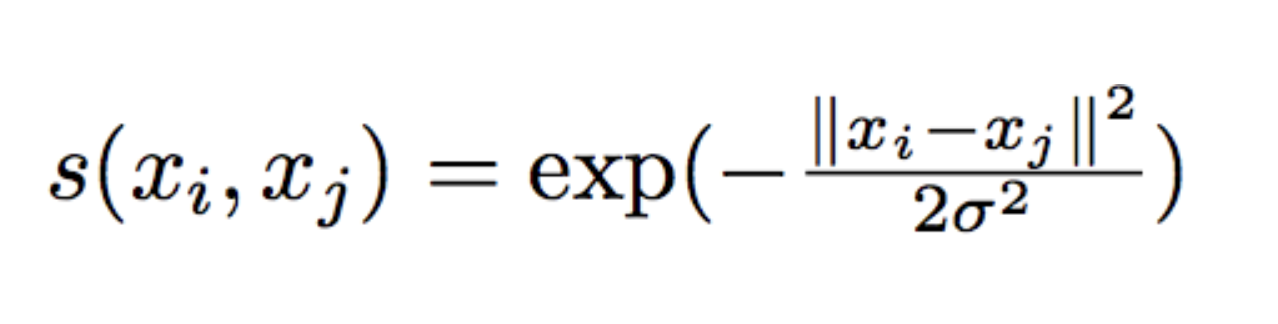
\includegraphics[width=0.5\textwidth]{images/spectral_gaussian.PNG} \newline
 The Gaussian similarity metric - where the parameter Sigma controls the width of the neighbourhood like the parameter Epsilon does in the Epsilon-neighbourhood graph. \newline

2.	Projecting the data onto a lower Dimensional Space: This step is done because it is possible that data points of the same cluster may be far away in the given dimensional space. That is why the goal is to transform the space so that when the two points are close, they should always be in the same cluster and in case they are far away from each other, they should be in different clusters. For the low-dimensional-space a Graph Laplacian Matrix is being used. The purpose of computing the Graph Laplacian is to find eigenvalues and eigenvectors. To compute it, the degree of a node needs to be defined. The degree of the ith node is given by \newline

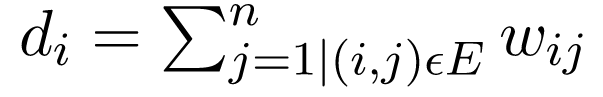
\includegraphics[width=0.5\textwidth]{images/spectral_degree.png}

Note that wi,j, is the edge between the nodes i and j as defined in the adjacency matrix above. The degree matrix is defined as follows \newline

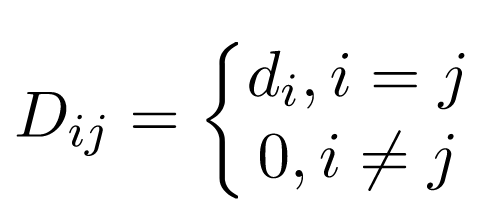
\includegraphics[width=0.3\textwidth]{images/spectral_degree_matrix.png}

Thus the Graph Laplacian Matrix is defined as: L = D – A, where A stands for the adjacency matrix and D stands for the degree matrix.
Afterwards the Matrix is being normalized for mathematical efficiency. The eigenvalues or rather the eigenvectors are calculated, to reduce the dimensions. If the number of clusters is k then the first eigenvalues and their eigen-vectors are taken and stacked into a matrix such that the eigen-vectors are the columns \cite{spectral-website}. \newline

3.	Clustering the Data: In this step the reduced data is being clustered by using any traditional clustering technique – typically K-Means Clustering. First, each node is assigned a row of the normalized of the Graph Laplacian Matrix. Afterwards, the data is clustered using any traditional technique. \newline

As Luxburg mentions in \cite{von2007tutorial}, Spectral Clustering helps creating more accurate clusters in comparisons to other clustering algorithms such as the K-Means Clustering. But on the other hand, using K-means clustering in the final steps implies that the clusters are not always the same. They may vary depending on the choice of the initial centroids \cite{spectral-website}. Additionally, Spectral Clustering is computationally expensive for large datasets. The reason for that is that eigenvalues and eigenvectors need to be computed and then clustering is being done on these vectors. For large data sets this may increase time complexity \cite{spectral-website}. \newline
If there are n data points, Spectral Clustering results in a complexity of O(n\textsuperscript{3}). That means  given a data set consisting of n data points, spectral clustering algorithms form an n × n affinity matrix and compute eigenvectors of this matrix, an operation that has a computational complexity of O(n\textsuperscript{3}) in general. For applications with n on the order of thousands, spectral clustering methods begin to become infeasible, and problems with n in the millions are out of reach. [30] \newline
